\label{appendix:crystal-facets}
% ``This surface consists of (111) terraces (three close-packed rows wide) and intrinsic (100) steps, which run parallel to the [011] direction. The close-packed atom rows located at the step edges are characterized by
%a nearest-neighbor distance of \SI{2.55}{\angstrom}  for Cu and of \SI{2.89}{\angstrom} for Ag, whereas the intrinsic step
%spacing is \SI{6.25}{\angstrom} for Cu and \SI{7.08}{\angstrom} for Ag. The surface symmetry is described by a primitive
%rectangular unit cell (cf. Figure 3.1a). The (111) terraces and the micro facets which represent the intrinsic (100) steps are tilted by \SI{19.5}{\degree}, respectively, to macroscopic (211) surface, which can be seen in the side view of the hard-sphere model in the upper panel of Figure 3.1a. The interlayer spacing for this surface is \SI{0.74}{\angstrom} for Cu and \SI{0.83}{\angstrom} for Ag.''
%
%``The (311) surface consists also of (111) terraces (two close-packed rows wide) and intrinsic (100) steps.''\cite[29ff]{riemann_ionic_2002, ma_interplay_2016, liu_oxygen_2014}

\begin{figure}\centering
	\subfigure[111]{
		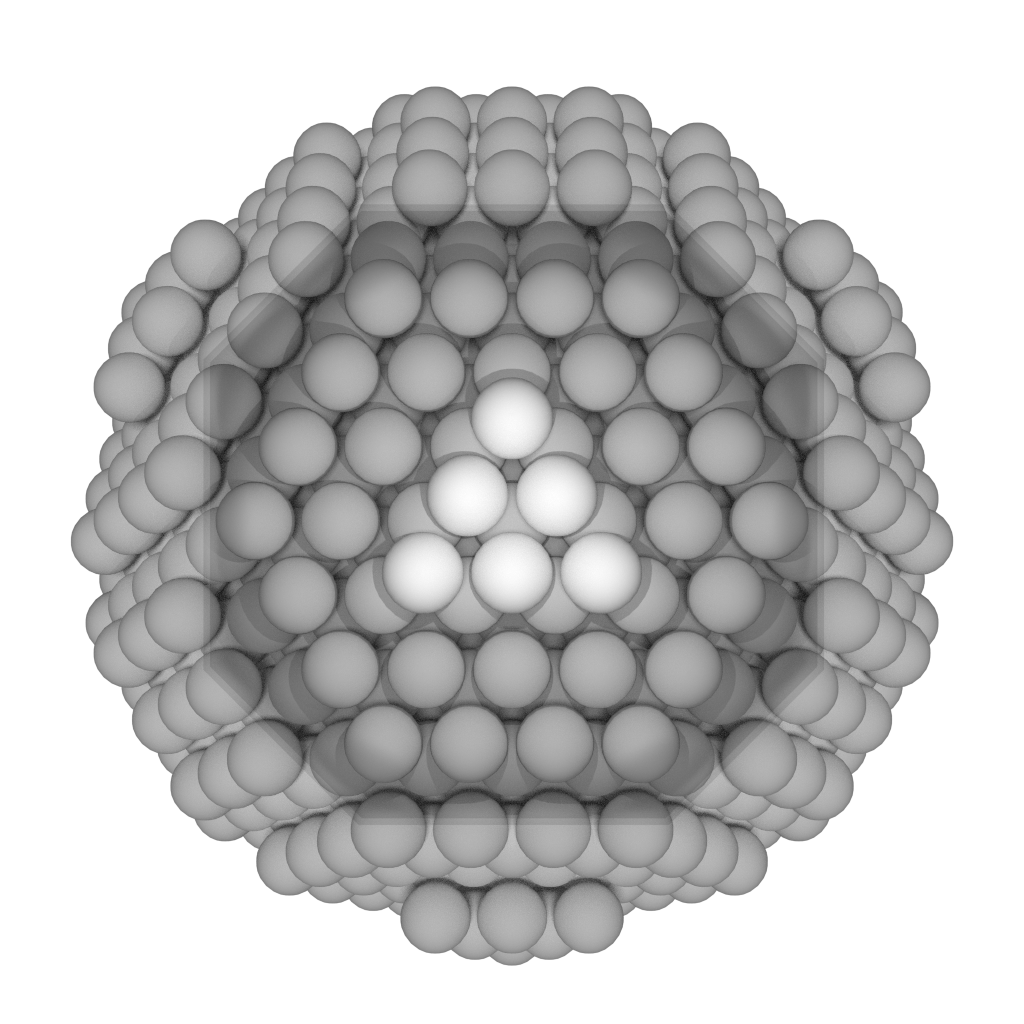
\includegraphics[width=0.2\textwidth]{./images/fcc-111-persp}
		\label{fig:crystal-facet-111}	
	} \quad%
	\subfigure[100]{
		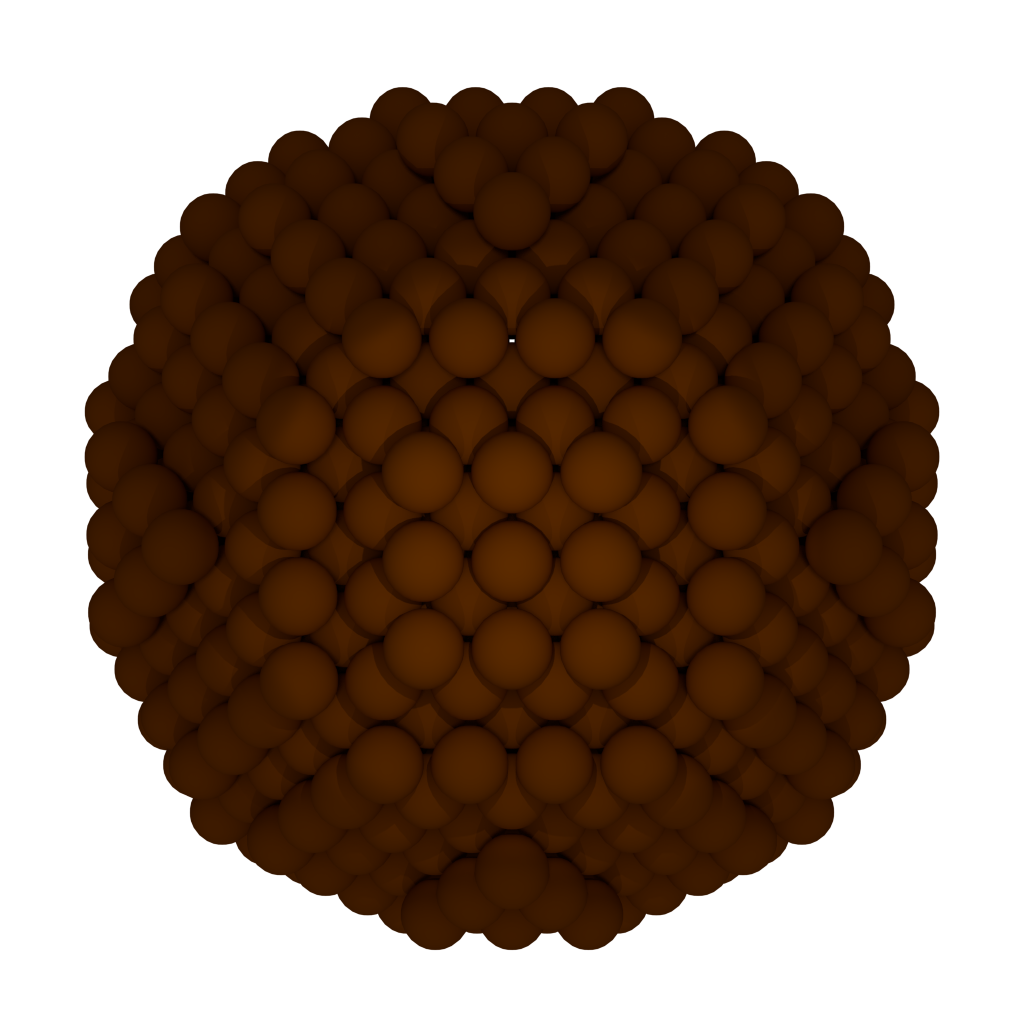
\includegraphics[width=0.2\textwidth]{./images/fcc-100-persp}
		\label{fig:crystal-facet-100}	
	} \quad%
	\subfigure[110]{
		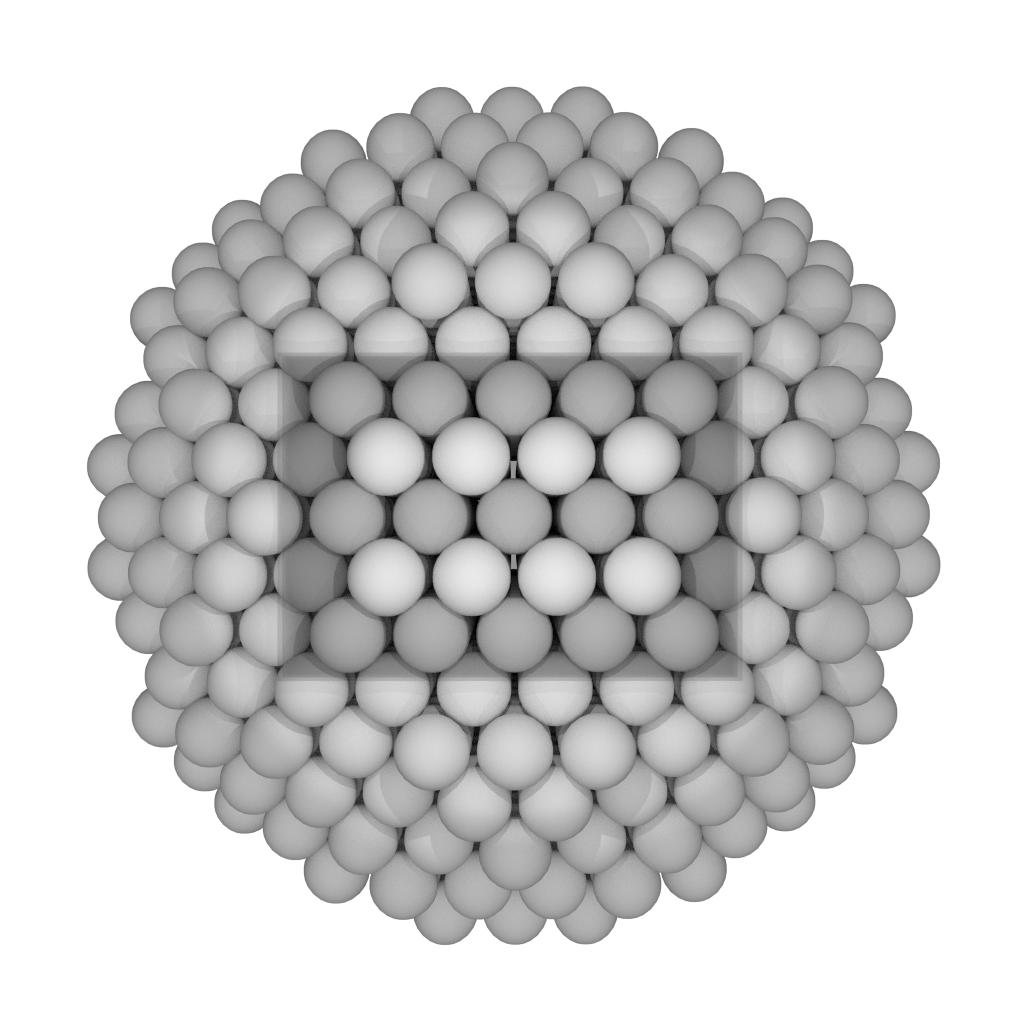
\includegraphics[width=0.2\textwidth]{./images/fcc-110-persp}
		\label{fig:crystal-facet-110}
	} \\
	\subfigure[311]{
		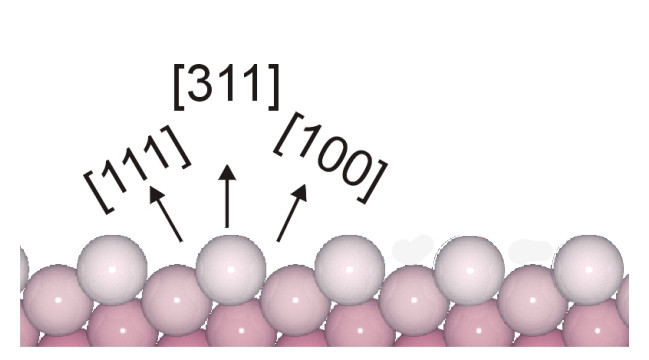
\includegraphics[width=0.2\textwidth]{./images/riemann-311-side}
		\label{fig:crystal-facet-311}	
	} \quad%
	\subfigure[211]{
		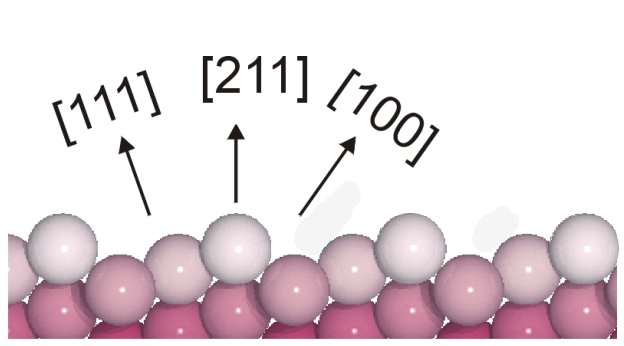
\includegraphics[width=0.2\textwidth]{./images/riemann-211-side}
		\label{fig:crystal-facet-211}	
	} \quad%
	\subfigure[221]{
		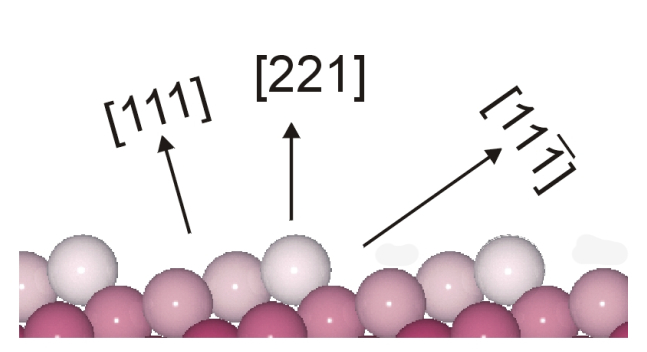
\includegraphics[width=0.2\textwidth]{./images/riemann-221-side}
		\label{fig:crystal-facet-221}
	}\quad
	\caption{Hard sphere models of different surface facets for a fcc crystal. \subref{fig:crystal-facet-111}-\subref{fig:crystal-facet-110} Same fcc crystalline cluster, viewed along the different surface normal of surface orientations (111), (110) \& (100). Terraces are parallel to the paper plane. \subref{fig:crystal-facet-311}-\subref{fig:crystal-facet-211} Higher order facets are shown from the side as they may be present on an unordered polycrystalline surface. 4(311), (211) \& (221) consist of (111) terraces separated by steps that form a regular stepped surface.
		\textbf{311}: (100) steps run parallel to [$0 \bar 1 1$], rhombic unit cell. Terrace is \SI{4,23}{\angstrom} (two close-packed rows) wide and inclined by \SI{33,5}{\deg}, steps by \SI{146,4}{\deg} with respect to the surface normal.
		\textbf{211}: (100) steps run parallel to [$0 1 \bar 1$] crystal direction. Rectangular unit cell. Terraces are four close-packed row wide (\SI{7,66}{\angstrom}) and inclined by \SI{19,5}{\deg}, steps by \SI{35,3}{\deg} with respect to the 221 surface normal. \SI{0,74}{\angstrom} interlayer spacing.
		\textbf{221}: (111) steps parallel to [$\bar 1 1 0$]. Steps go up in [$\bar 1 \bar 1 4$], rectangular unit cell. Terraces are \SI{7,66}{\angstrom} wide, inclined by \SI{15,8}{\deg}, steps by \SI{54,7}{\deg} with respect to the [221] surface normal. \SI{0,6}{\angstrom} interlayer spacing. Lower graphics row adapted from \cite{riemann_ionic_2002}.
	}
	\label{tab:step-heights}
\end{figure}

\paragraph{surface structure of \textit{h}-BN on Cu-foil}
During experiments some ``new'' structure appeared (compare figure \ref{fig:tpcn-on-cu-foil}).
The apparent height change between the both terraces is \SI{130}{\pico \meter} separated by a slim trench that is slightly lower than the right terrace (\SI{50}{\pico \meter}). The parallel stripes have an apparent corrugation of \SI{25}{\pico \meter} and are separated \SI{70}{\pico \meter} from each other and cover the whole image. 

The adsorbed TPCN molecules show different apparent heights in their molecular center. Some fragmented and heavily deformed molecules are visible.

\begin{figure}
	\centering
	\subfigure[Molecules on copper foil surface - supposed be be covered with \textit{h}-BN, maybe just free (maybe facetted) copper. Stripes not visible on the lower teracce, although present in the same orientation.]{
		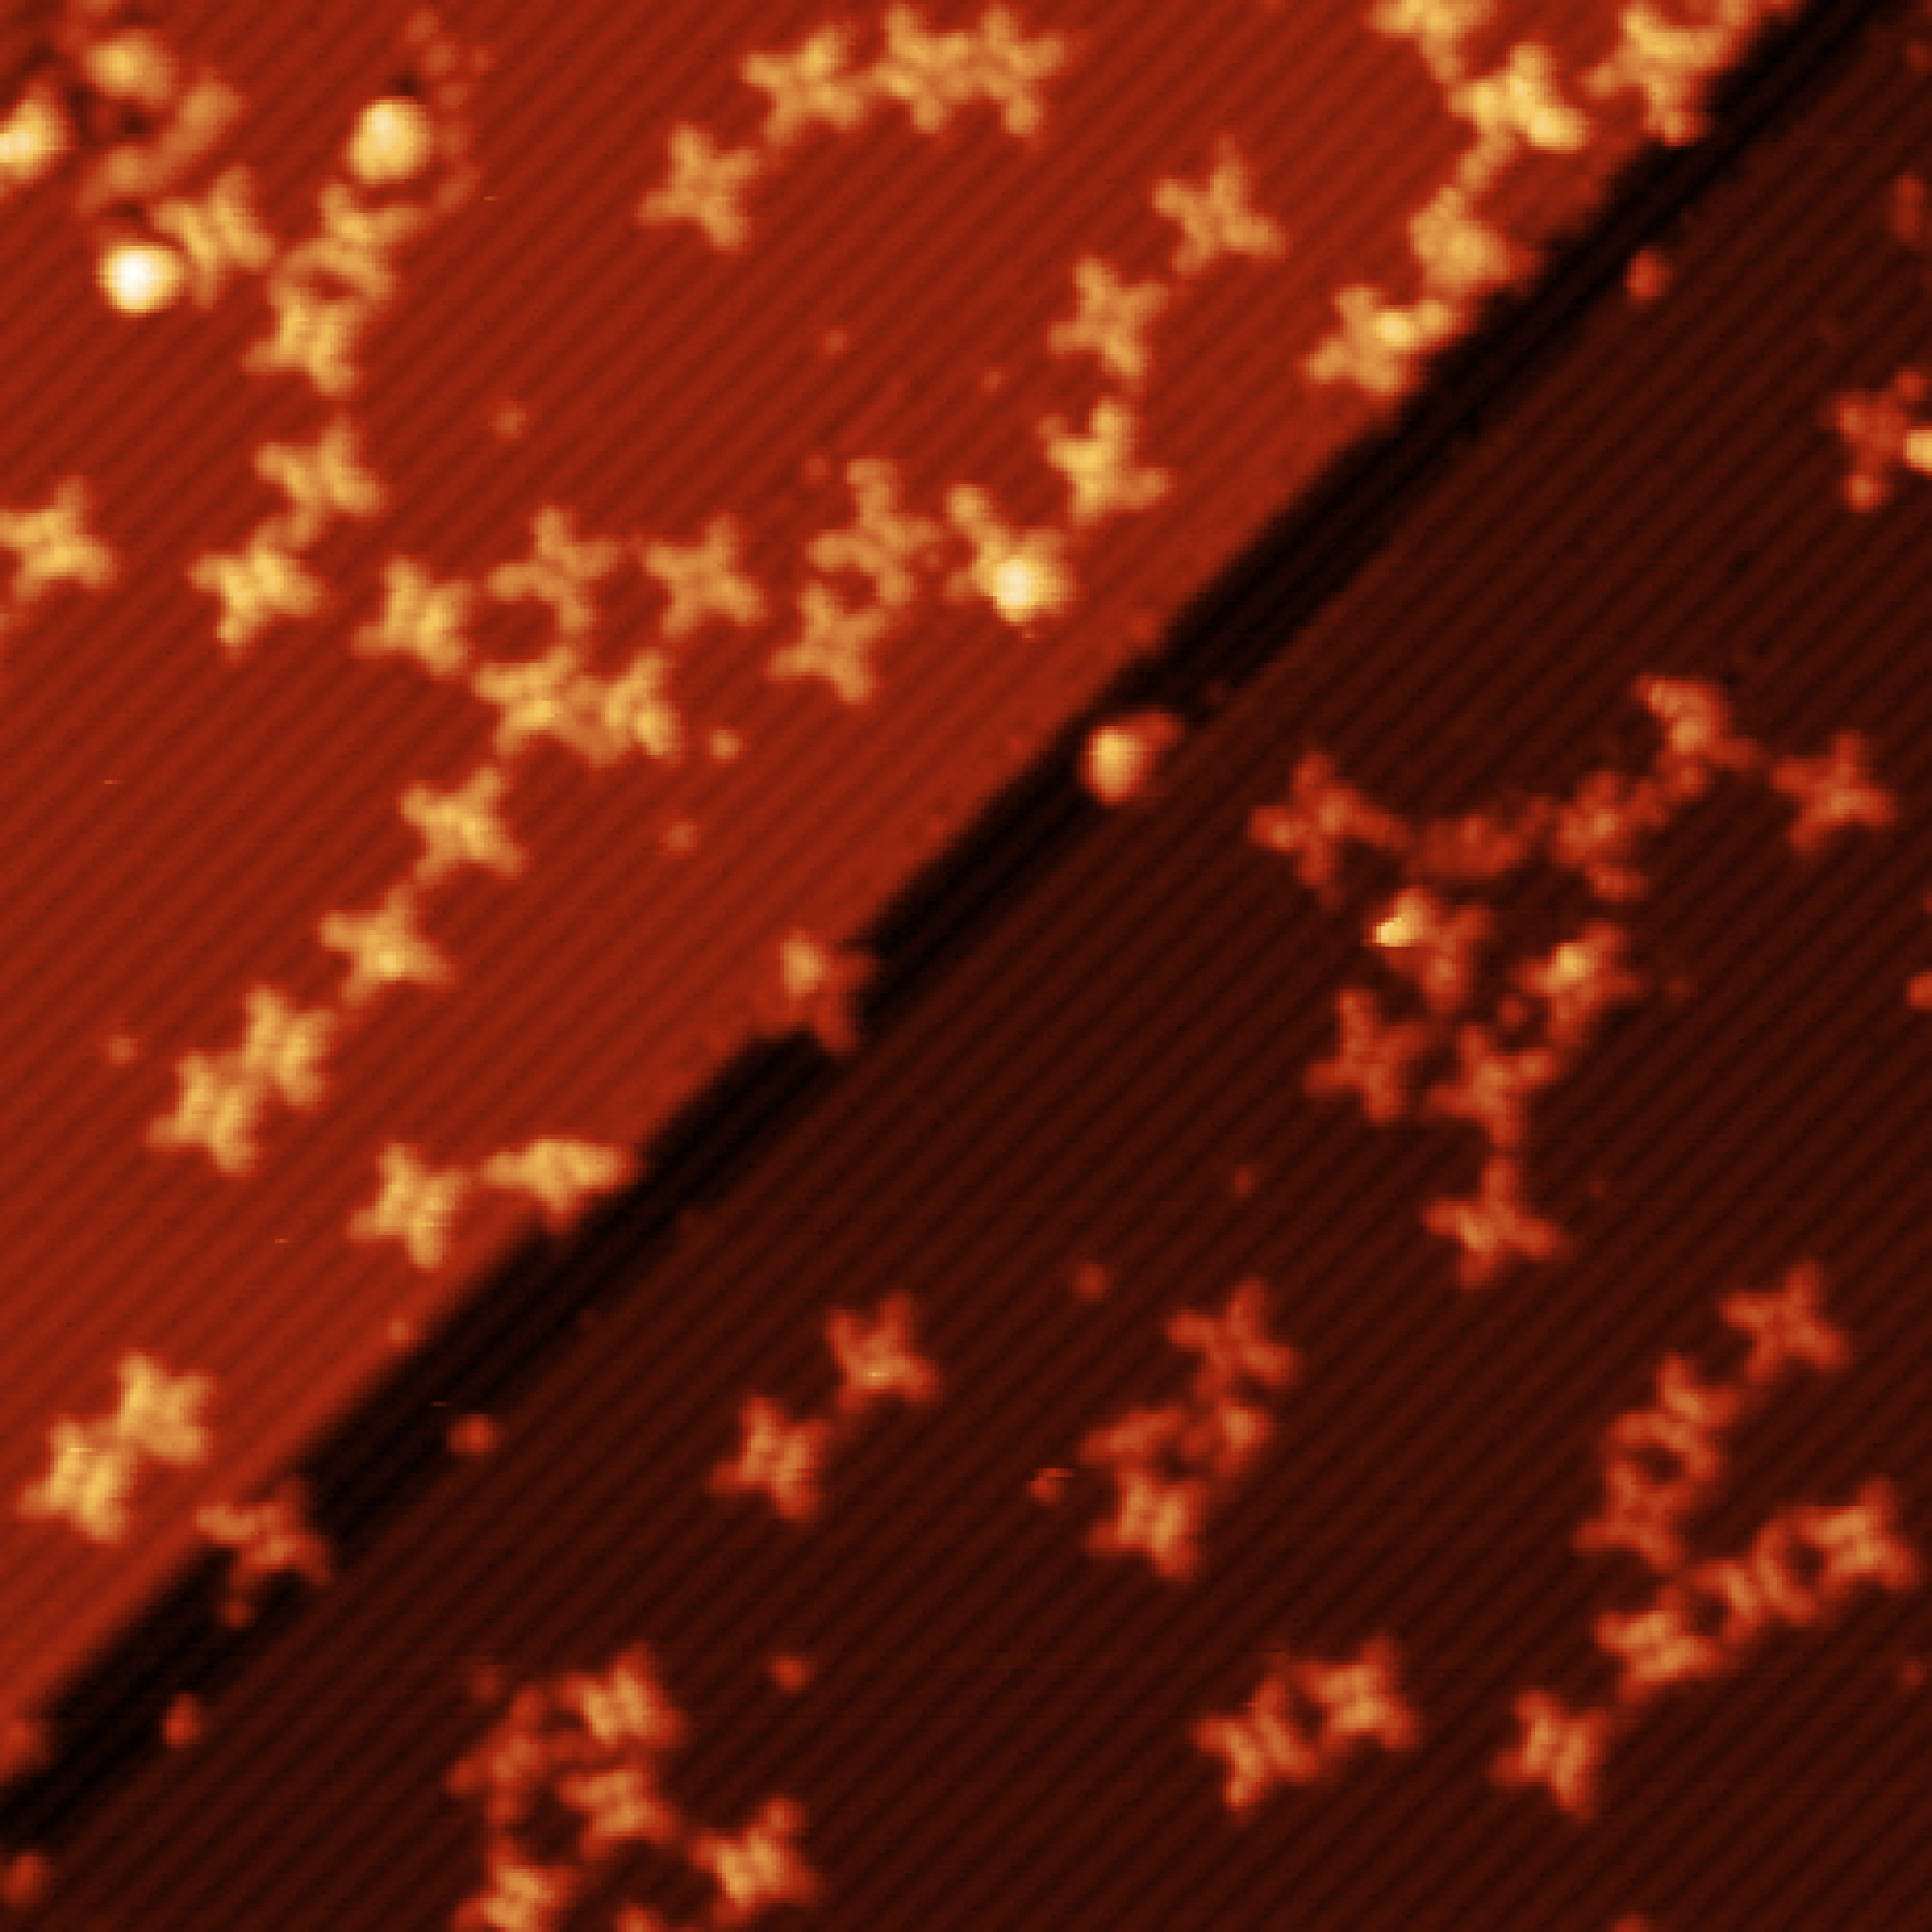
\includegraphics[width=0.45\textwidth]{./images/F150810-113456}
		\label{fig:tpcn-on-cu-foil-stm}
	} \quad
	\subfigure[Line spectrum across the step shown in \subref{fig:tpcn-on-cu-foil-stm} perpendicular to the trench. No molecules were crossed.]{
		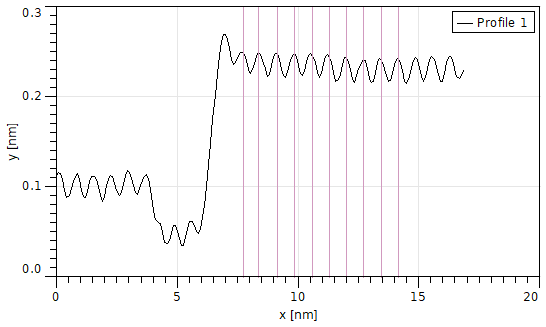
\includegraphics[width=0.45\textwidth]{./images/F150810-113456-line-spectra}
		\label{fig:tpcn-on-cu-foil-spectrum}
	}
	\caption{Surface structure of copper foil after deposition of TPCN molecules. Two terraces are visible, both covered with linear stripes - oxygen over layer (2x1)?- cu reconstruction? - maybe some very small (\SI{0.75}{\nm}) linear moire on a Cu(100) facet? Noise can be excluded due to the fact that the stripes do not occur on the molecules, but only on the substrate. Adsorbed TPCN molecules appear as cross shaped protrusions. Many deformed molecular cores visible throughout the image $\rightarrow$ strong substrate interaction $\rightarrow$ no \textit{h}-BN! Line spectrum shown in \subref{fig:tpcn-on-cu-foil-spectrum} indicating a period of \SI{70}{\pico \meter}. Imaging parameters: 		
		\subref{fig:tpcn-on-cu-foil-stm} 
		\SI{1.26}{\volt}, \SI{0.04}{\nano\ampere}, 
		color scale \SIrange{0}{0.8}{\nano \meter}, 
		Image width: \SI{40}{\nano \meter} }
	\label{fig:tpcn-on-cu-foil}
\end{figure}